{	% Background Image
\usebackgroundtemplate{
	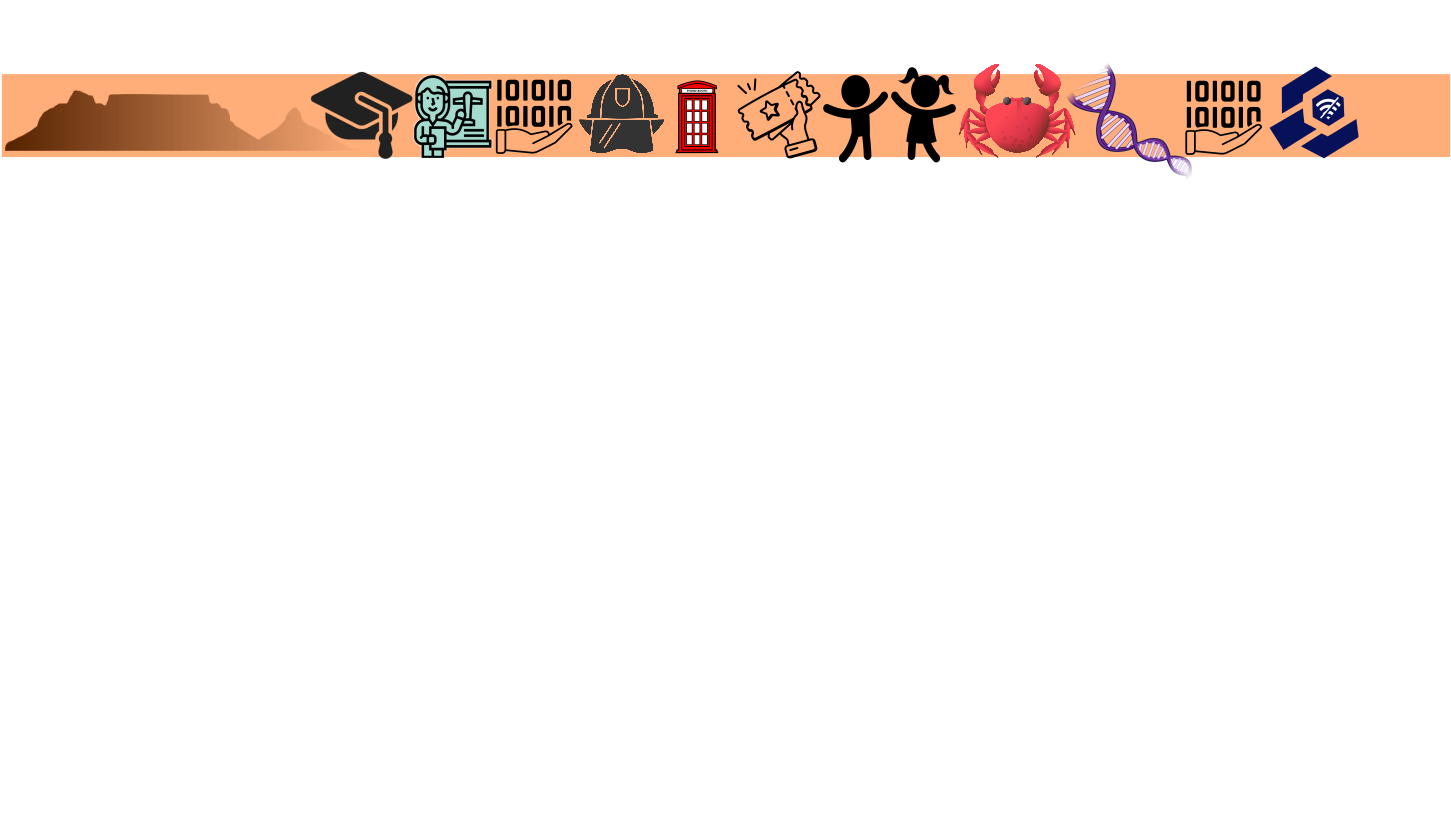
\includegraphics[width=\paperwidth]{images/TitleSlideBackground_red.png}
}
\begin{frame}

	

	
	%%%%%%%%%% Title slide code %%%%%%%%%%%
	\begin{tikzpicture}[remember picture,overlay]
	
		
		% Title & Subtitle
		\node
		[
		    above=-0.7cm,
		    align=center,
		    draw=carpblue,
		    left color=carpblue!50,
		    right color=carpblue!5,
		    shading angle=60,
		    double,
		    double distance=0.1cm,
		    inner xsep=15pt,
		    inner ysep=10pt, 
		    minimum width=0.7\textwidth,
		    text width=0.6\textwidth
		] (title) at (current page.center)
		{
		    \LARGE \myTitle  \\[5pt]
		    \small \mySubTitle
		};
		
		% Author 
		\node[ below=0.5cm] (author) at (title.south){\myAuthor};
		
		% Author 
		\node[ below=0.25cm] (affiliate) at (author.south){\small \myAffiliate};
		
		% Date
		\node[below=0.25cm] (date) at (affiliate.south){\large \myDate};
		
		% Logo
		\node
		[
		    below right =0.25cm and 0.5cm
		] at (current page.north west)
		{
		    \myLogo
		};
	
	\end{tikzpicture}
	
	
		\note{
		Almost everyone I met and ask about how they got to be an RSE will start by saying that they got into it in a bit of a weird way. Since just about everybody says that, I have come to the conclusion that there isn't an ordinary way to become an RSE. So I thought I'll share, with you, my story, the things I've done, the things I have learnt. If you're on the senior side of research software engineering you might nod your head in agreement and if you are on the junior side you might pick up on a few things to do or not to do.
		
		I'll talk a bit about my life before being an RSE and then about our RSE team in Newcastle, my IRS (the old SSI) fellowship, CarpentriesOffline and running Carpentries workshops.
		
		
	}

\end{frame}
}